\documentclass[12pt]{article}

\usepackage{sbc-template}
\usepackage[utf8]{inputenc}
\usepackage[T1]{fontenc}
\usepackage[english,brazilian]{babel}
\usepackage{graphicx,url}
\usepackage{booktabs}
\usepackage{tikz}
\usetikzlibrary{arrows.meta,positioning}

\sloppy
\hyphenation{SMILES}

% Números citados no texto, gerados por scripts/rn_report.py a partir de results/rn_dados.json.
% Gerado por scripts/rn_report.py a partir de report/results/rn_dados.json; não editar.
\newcommand{\rnLinhas}{4.269}
\newcommand{\rnAprovados}{62,2}
\newcommand{\rnNegativos}{28}
\newcommand{\rnRegraBase}{95,4}
\newcommand{\rnAprovAbaixo}{10}
\newcommand{\rnAprovAcima}{99,5}
\newcommand{\rnAprovPrazoDois}{48}
\newcommand{\rnAprovPrazoQuatro}{57}
\newcommand{\rnCorrScore}{0,77}
\newcommand{\rnCorrPrazo}{$-$0,11}
\newcommand{\rnCorrRendaValor}{0,93}
\newcommand{\rnCorrRendaLuxo}{0,93}
\newcommand{\rnTreino}{3.415}
\newcommand{\rnTeste}{854}
\newcommand{\rnPrimeiraAcc}{92,3}
\newcommand{\rnPrimeiraEpocas}{90}
\newcommand{\rnSemPadAcc}{59,5}
\newcommand{\rnSemPadSd}{3,1}
\newcommand{\rnSemPadAuc}{51,0}
\newcommand{\rnComPadAcc}{93,9}
\newcommand{\rnComPadSd}{0,7}
\newcommand{\rnCombinacoes}{24}
\newcommand{\rnCombinacoesArv}{30}
\newcommand{\rnSeedsTaxa}{10}
\newcommand{\rnSeedsDuas}{9}
\newcommand{\rnSeedsTrintaDezesseis}{7}
\newcommand{\rnEpocasMin}{40}
\newcommand{\rnEpocasMed}{66,5}
\newcommand{\rnEpocasMax}{121}
\newcommand{\rnAccMaj}{62,2}
\newcommand{\rnSdMaj}{0,0}
\newcommand{\rnAucMaj}{50,0}
\newcommand{\rnErrosMaj}{323,0}
\newcommand{\rnAccRegra}{95,5}
\newcommand{\rnSdRegra}{0,6}
\newcommand{\rnAucRegra}{96,2}
\newcommand{\rnErrosRegra}{38,8}
\newcommand{\rnAccLog}{91,9}
\newcommand{\rnSdLog}{1,1}
\newcommand{\rnAucLog}{97,0}
\newcommand{\rnErrosLog}{69,5}
\newcommand{\rnAccArv}{98,1}
\newcommand{\rnSdArv}{0,4}
\newcommand{\rnAucArv}{98,7}
\newcommand{\rnErrosArv}{16,0}
\newcommand{\rnAccRF}{98,3}
\newcommand{\rnSdRF}{0,4}
\newcommand{\rnAucRF}{99,8}
\newcommand{\rnErrosRF}{14,5}
\newcommand{\rnAccRede}{96,4}
\newcommand{\rnSdRede}{1,1}
\newcommand{\rnAucRede}{99,3}
\newcommand{\rnErrosRede}{30,9}
\newcommand{\rnAccRegraEn}{95.5}
\newcommand{\rnAccLogEn}{91.9}
\newcommand{\rnAccArvEn}{98.1}
\newcommand{\rnAccRedeEn}{96.4}
\newcommand{\rnLinhasEn}{4,269}
\newcommand{\rnTreinoArvMs}{3,7}
\newcommand{\rnTreinoRedeMs}{183}
\newcommand{\rnTreinoRFMs}{490}
\newcommand{\rnBuscaRede}{23,5}
\newcommand{\rnBuscaArv}{0,65}
\newcommand{\rnPrevRFMs}{15}
\newcommand{\rnPrevRedeMs}{0,6}
\newcommand{\rnRazaoTreino}{50}
\newcommand{\rnRazaoBusca}{36}
\newcommand{\rnDifRedeRegra}{0,9}
\newcommand{\rnSeedsRedeRegra}{8}
\newcommand{\rnDifRedeLog}{4,5}
\newcommand{\rnSeedsRedeLog}{10}
\newcommand{\rnDifRedeArv}{$-$1,7}
\newcommand{\rnSeedsRedeArv}{0}
\newcommand{\rnDifRedeRF}{$-$1,9}
\newcommand{\rnSeedsRedeRF}{1}
\newcommand{\rnDifRegraLog}{3,6}
\newcommand{\rnSeedsRegraLog}{10}
\newcommand{\rnDifArvRegra}{2,7}
\newcommand{\rnSeedsArvRegra}{10}
\newcommand{\rnDifRFArv}{0,2}
\newcommand{\rnSeedsRFArv}{5}
\newcommand{\rnParadaLentaDez}{37}
\newcommand{\rnParadaAccLentaDez}{92,1}
\newcommand{\rnParadaLentaTrinta}{217}
\newcommand{\rnParadaAccLentaTrinta}{95,5}
\newcommand{\rnParadaRapidaDez}{54}
\newcommand{\rnParadaAccRapidaDez}{96,8}
\newcommand{\rnParadaRapidaTrinta}{94}
\newcommand{\rnParadaAccRapidaTrinta}{97,1}
\newcommand{\rnMelhorLenta}{96,5}
\newcommand{\rnMelhorRapida}{97,4}
\newcommand{\rnNeurUm}{93,4}
\newcommand{\rnNeurQuatro}{97,2}
\newcommand{\rnNeurSessentaQuatro}{95,4}
\newcommand{\rnNeurOitoDuas}{98,0}
\newcommand{\rnErrosRedeSeed}{23}
\newcommand{\rnErrosArvSeed}{15}
\newcommand{\rnPedidosFaixa}{73}
\newcommand{\rnErrosRedeFaixa}{9}
\newcommand{\rnErrosArvFaixa}{1}
\newcommand{\rnExcecao}{52}
\newcommand{\rnErrosRedeExc}{8}
\newcommand{\rnErrosArvExc}{12}
\newcommand{\rnInterRede}{24}
\newcommand{\rnInterArv}{1}
\newcommand{\rnFPRedeSeed}{11}
\newcommand{\rnFNRedeSeed}{12}
\newcommand{\rnFPRedeMed}{16,5}
\newcommand{\rnFNRedeMed}{14,4}
\newcommand{\rnTaxaFPRede}{5,1}
\newcommand{\rnTaxaFNRede}{2,7}
\newcommand{\rnSeedsFNRede}{2}
\newcommand{\rnFPArvSeed}{10}
\newcommand{\rnFNArvSeed}{5}
\newcommand{\rnFPArvMed}{9,4}
\newcommand{\rnFNArvMed}{6,6}
\newcommand{\rnTaxaFPArv}{2,9}
\newcommand{\rnTaxaFNArv}{1,2}
\newcommand{\rnSeedsFNArv}{2}
\newcommand{\rnTesteRej}{323}
\newcommand{\rnTesteAprov}{531}
\newcommand{\rnRejeitadosBase}{1.613}
\newcommand{\rnRazaoClasses}{1,6}


\title{Redes neurais na aprovação de empréstimos: comparação com árvore de decisão e modelos de referência}

\author{Bernan R. do Nascimento\inst{1}, Paulo E. R. Araujo\inst{1}, Thiago R. P. de Carvalho\inst{1}}

\address{Universidade Federal do Piauí (UFPI)\\
  Programa de Pós-Graduação em Ciência da Computação -- Teresina -- PI -- Brasil\\
  PPGCC010 -- Aprendizagem de Máquina (2026.2) -- Prof. Vinicius Ponte Machado
  \email{bernanr7@gmail.com, pauloaraujo@ufpi.edu.br}
  \email{thiago.rafael.pc@gmail.com}
}

\begin{document}

\maketitle

\begin{abstract}
  We predict whether a loan application is approved from 11 attributes of the application and the
  applicant, on a public dataset of \rnLinhasEn{} applications, and use it to study how a multilayer
  perceptron is trained and to compare it with simpler models, including execution time. The network
  reaches \rnAccRedeEn\%, above a one-threshold rule (\rnAccRegraEn\%) and logistic regression
  (\rnAccLogEn\%) but below a decision tree (\rnAccArvEn\%), which also trains about \rnRazaoTreino{}
  times faster. The labels follow a step on the credit score: the tree draws it with one cut, while the
  network approximates it with a ramp, where its errors concentrate.
\end{abstract}

\begin{resumo}
  Prevemos se um pedido de empréstimo foi aprovado a partir de 11 atributos do pedido e de quem o fez,
  numa base pública de \rnLinhas{} pedidos, e a usamos para estudar o treino de uma rede neural e
  compará-la com modelos mais simples, incluindo o tempo de execução. Sem padronização dos atributos, a
  rede não aprende (\rnSemPadAcc\%). Com ela, uma rede neural (perceptron de múltiplas camadas) acerta
  \rnAccRede\%, acima de uma regra de um corte (\rnAccRegra\%) e da regressão logística (\rnAccLog\%),
  mas abaixo da árvore de decisão (\rnAccArv\%), que ainda treina cerca de \rnRazaoTreino{} vezes mais
  rápido. Os rótulos seguem um degrau no score de crédito: a árvore o representa com um corte, e a rede
  o aproxima com uma rampa, onde se concentram seus erros.
\end{resumo}

\section{Introdução}

Este trabalho trata da previsão de aprovação de pedidos de empréstimo: dado um pedido, descrito por 11 atributos do pedido e de quem o fez, prever se ele foi aprovado. A base, publicada no Kaggle~\cite{kaggle:loan}, é pequena, sem valores ausentes, e o rótulo depende quase só do score de crédito. Ela serve para estudar o treino de uma rede neural (padronização, número de neurônios, épocas e parada antecipada) e para comparar a rede com modelos mais simples num caso em que a forma da regra que gerou os rótulos é conhecida.

O modelo principal é uma rede neural do tipo perceptron de múltiplas camadas (MLP), comparada com cinco modelos de referência: a classe majoritária, uma regra de um corte, a regressão logística, a árvore de decisão e a Random Forest. Além da acurácia, registramos o tempo de treino, de busca de hiperparâmetros e de previsão de cada modelo. As contribuições são:
\begin{itemize}
  \item uma análise exploratória que mostra que os rótulos seguem quase um degrau no score de crédito, com uma exceção para prazos curtos (Seção~\ref{sec:rn_eda});
  \item um estudo do treino da rede: o efeito da padronização, do número de neurônios e da paciência da parada antecipada (Seção~\ref{sec:rn_resultados});
  \item uma comparação da rede com os modelos de referência em 10 seeds, com acurácia, F1 macro, AUC e tempo num único núcleo, que mostra quando a rede não compensa;
  \item uma análise de onde cada modelo erra, que liga os erros da rede à rampa com que ela aproxima o degrau.
\end{itemize}

\section{Fundamentação}

\textbf{Redes neurais.} Um neurônio artificial calcula uma soma ponderada das entradas, mais um viés, e aplica a ela uma função de ativação. Com a sigmoide, que leva qualquer número a um valor entre 0 e 1, um único neurônio é a regressão logística. O perceptron de múltiplas camadas (MLP) empilha camadas de neurônios entre a entrada e a saída, as camadas ocultas; com a ativação ReLU, $\max(0, z)$~\cite{nair:10}, elas permitem fronteiras de decisão não lineares. Os pesos começam sorteados e são ajustados pela retropropagação do erro~\cite{rumelhart:86}: a cada lote de exemplos, calcula-se quanto cada peso contribuiu para a perda (aqui, a entropia cruzada) e move-se o peso no sentido de reduzi-la, com um passo dado pela taxa de aprendizado. O otimizador Adam~\cite{kingma:15} adapta esse passo para cada peso. Uma época é uma passada completa pelo treino. Como o passo é o mesmo para entradas de escalas muito diferentes, os atributos costumam ser padronizados antes~\cite{lecun:98}. Treinar por épocas demais leva a rede a se ajustar a detalhes do treino; a parada antecipada~\cite{prechelt:98} separa uma parte do treino como validação e interrompe o treino quando o desempenho nela para de melhorar. Em dados tabulares, modelos de árvore ainda costumam superar redes neurais, em parte porque as redes tendem a aprender funções suaves e as árvores representam bem relações irregulares, como degraus~\cite{grinsztajn:22}.

\textbf{Modelos de referência.} O CART~\cite{breiman:84} divide o espaço de atributos de forma recursiva, em cada nó escolhendo o limiar de um atributo que mais reduz a impureza (Gini ou entropia); a vantagem é a legibilidade das regras. Uma árvore de profundidade 1 é uma \emph{regra de um corte}: um único atributo comparado com um único limiar. A Random Forest~\cite{breiman:01} treina muitas árvores, cada uma numa amostra com reposição do treino (\emph{bootstrap}) e com sorteio dos atributos de cada nó, e a previsão é a média dos votos. A regressão logística, como visto acima, equivale a uma rede de um único neurônio.

\section{Dados e curadoria}\label{sec:rn_dados}

A base é o \emph{Loan-Approval-Prediction-Dataset}, publicado no Kaggle~\cite{kaggle:loan}: \rnLinhas{} pedidos, cada um com um identificador, 11 atributos e o rótulo (aprovado ou rejeitado). A Tabela~\ref{tab:rn_atributos} lista os atributos com os nomes usados neste trabalho. A página não informa a moeda; como o score é o do CIBIL, o birô de crédito da Índia, os valores devem estar em rúpias. Isso não afeta os modelos, que só comparam valores entre si.

\begin{table}[ht]
\centering
\caption{Atributos da base de empréstimos: nome no arquivo original, nome usado neste trabalho e faixa de valores. Valores em dinheiro em milhões, na moeda da base.}
\label{tab:rn_atributos}
\footnotesize
\begin{tabular}{lll}
\toprule
Coluna original & Nome neste trabalho & Valores \\
\midrule
\texttt{no\_of\_dependents} & dependentes & 0 a 5 \\
\texttt{education} & graduado & 1 = \emph{Graduate}, 0 = \emph{Not Graduate} \\
\texttt{self\_employed} & autônomo & 1 = \emph{Yes}, 0 = \emph{No} \\
\texttt{income\_annum} & renda anual & 0,2 a 9,9 \\
\texttt{loan\_amount} & valor do empréstimo & 0,3 a 39,5 \\
\texttt{loan\_term} & prazo (anos) & 2 a 20, de 2 em 2 \\
\texttt{cibil\_score} & score de crédito & 300 a 900 \\
\texttt{residential\_assets\_value} & patrimônio residencial & 0 a 29,1 \\
\texttt{commercial\_assets\_value} & patrimônio comercial & 0 a 19,4 \\
\texttt{luxury\_assets\_value} & bens de luxo & 0,3 a 39,2 \\
\texttt{bank\_asset\_value} & saldo bancário & 0 a 14,7 \\
\texttt{loan\_status} & aprovado (rótulo) & 1 = \emph{Approved}, 0 = \emph{Rejected} \\
\bottomrule
\end{tabular}
\end{table}

A curadoria foi curta, porque a base não tem valores ausentes nem linhas repetidas. O arquivo baixado é conferido pelo seu \emph{hash} SHA-256, para garantir que todos os experimentos partem do mesmo arquivo. Os nomes de colunas e os textos vinham com espaços no início, que foram removidos. \rnNegativos{} pedidos tinham patrimônio residencial de $-$100 mil, um valor impossível. Como a taxa de aprovação nessas linhas (57\%) é próxima da geral (\rnAprovados\%), o valor parece um erro de digitação, e não um sinal sobre o pedido; as linhas foram mantidas e o valor foi trocado por 0, que já aparece em outros 45 pedidos. Por fim, os três textos (escolaridade, autônomo e situação) viraram 0 e 1.

\section{Análise exploratória}\label{sec:rn_eda}

\rnAprovados\% dos pedidos foram aprovados, cerca de \rnRazaoClasses{} aprovado para cada rejeitado: a base é moderadamente desbalanceada, e a acurácia sozinha engana, porque responder sempre ``aprovado'' já acerta \rnAprovados\%. Esse é o piso. Um atributo domina os demais: o score de crédito tem correlação de \rnCorrScore{} com a aprovação, enquanto o prazo tem \rnCorrPrazo{} e os outros nove ficam perto de zero. Os valores em dinheiro são redundantes entre si: a renda anual tem correlação de \rnCorrRendaValor{} com o valor do empréstimo e de \rnCorrRendaLuxo{} com os bens de luxo (Figura~\ref{fig:rn_corr}).

\begin{figure}[ht]
\centering
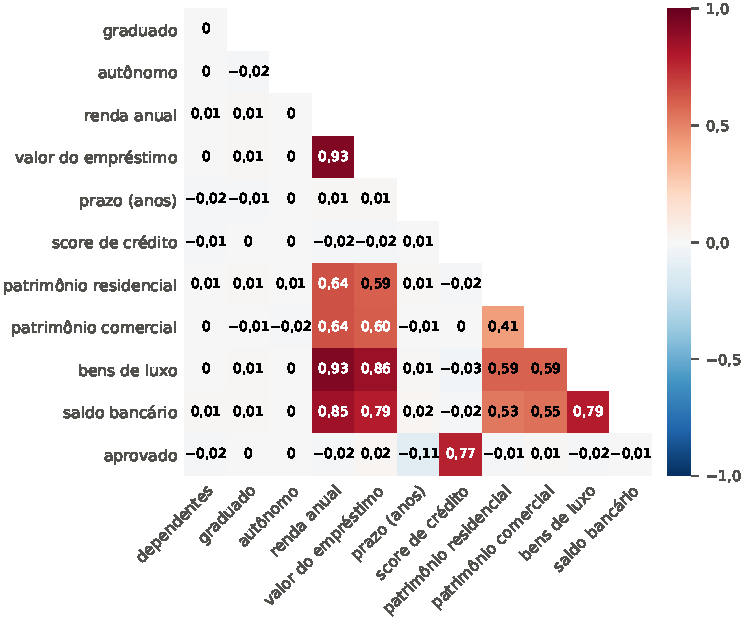
\includegraphics[width=.8\textwidth]{figures/rn_correlacao.pdf}
\caption{Correlação de Pearson entre os 11 atributos e a aprovação, na base inteira (\rnLinhas{} pedidos). Só o score de crédito se relaciona fortemente com a aprovação; os valores em dinheiro se correlacionam entre si e quase nada com o alvo.}
\label{fig:rn_corr}
\end{figure}

A Figura~\ref{fig:rn_score} mostra a forma dessa relação, e ela não é gradual: abaixo de 550 pontos, cerca de \rnAprovAbaixo\% dos pedidos são aprovados, em qualquer faixa; a partir de 550, \rnAprovAcima\%. A regra ``aprovar se o score for de pelo menos 550'' acerta \rnRegraBase\% da base. Os aprovados abaixo de 550 têm todos prazo de 2 ou 4 anos (\rnAprovPrazoDois\% e \rnAprovPrazoQuatro\% de aprovação nesses prazos); com prazos maiores, nenhum pedido abaixo de 550 foi aprovado. Os rótulos seguem, portanto, quase uma regra explícita: um degrau no score, com uma exceção para prazos curtos.

\begin{figure}[ht]
\centering
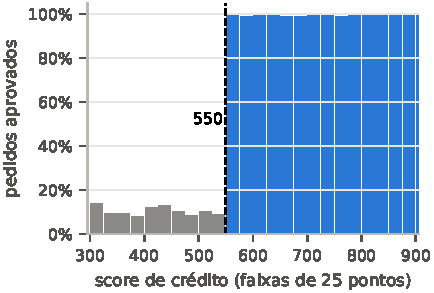
\includegraphics[width=.55\textwidth]{figures/rn_aprovacao_score.pdf}
\caption{Proporção de pedidos aprovados por faixa de 25 pontos de score de crédito. A linha tracejada marca 550.}
\label{fig:rn_score}
\end{figure}

A base parece sintética. O score e a renda se distribuem de forma quase uniforme: os quartis do score são 453, 600 e 748, contra 450, 600 e 750 de uma distribuição uniforme entre 300 e 900. Escolaridade e autônomo se dividem quase meio a meio. Com dados de crédito reais, seriam esperadas distribuições concentradas e uma relação mais gradual entre o score e a aprovação. Isso limita o alcance das conclusões (Seção~\ref{sec:limitacoes}).

\section{Metodologia}\label{sec:rn_metodo}

\textbf{Protocolo.} Os dados são divididos em treino (80\%, \rnTreino{} pedidos) e teste (20\%, \rnTeste), mantendo a proporção de aprovados, e o procedimento é repetido com 10 seeds (0 a 9), que mudam a divisão, as partes da validação cruzada e a semente dos modelos. Como a base não tem linhas repetidas, a divisão é estratificada simples. Quando um modelo tem hiperparâmetros a escolher, uma busca em grade com validação cruzada estratificada de 5 partes, feita só dentro do treino, escolhe a combinação de maior acurácia. No teste, reportam-se acurácia, F1 macro, a área sob a curva ROC (AUC) e, para a rede e a árvore, a matriz de confusão. O desbalanceamento é tratado pela divisão e pela validação estratificadas e por métricas que não favorecem a classe maior: o F1 macro, média simples do F1 das duas classes, a AUC, que não depende da proporção entre elas, e a matriz de confusão, que mostra o erro em cada uma. Não usamos reamostragem nem pesos por classe, porque a classe menor tem \rnRejeitadosBase{} pedidos e os modelos acertam bem as duas classes. A AUC usa a probabilidade prevista, e não a classe: é a chance de um pedido aprovado, sorteado ao acaso, receber probabilidade maior que um rejeitado. Ela mede, portanto, se o modelo ordena bem os pedidos, independentemente do corte em 50\%.

\textbf{Modelos de referência.} Cinco modelos servem de régua: a classe majoritária; a \emph{regra de um corte}, uma árvore de profundidade 1 que escolhe sozinha, no treino, o melhor atributo e o melhor limiar (escolheu o score e 549,5 nas 10 seeds); a regressão logística com padronização, que equivale a uma rede de um único neurônio; a árvore de decisão com busca em grade (critério, profundidade máxima e mínimo por folha, \rnCombinacoesArv{} combinações); e a Random Forest com 300 árvores.

\textbf{A rede neural.} A rede é um MLP do scikit-learn~\cite{pedregosa:11}: camadas ocultas com ativação ReLU~\cite{nair:10}, um neurônio de saída com sigmoide, que dá a probabilidade de aprovação, perda de entropia cruzada e otimizador Adam~\cite{kingma:15}. Antes da rede, cada atributo é padronizado (subtrai-se a média e divide-se pelo desvio padrão do treino, nunca do teste). O treino usa parada antecipada~\cite{prechelt:98}: 10\% do treino ficam de fora como validação, e o treino para quando a acurácia nessa validação passa um número fixo de épocas, a \emph{paciência}, sem melhorar. Usamos paciência de 30 épocas em vez das 10 do padrão do scikit-learn, pelo motivo mostrado na Seção~\ref{sec:rn_resultados}. A busca em grade cobre a arquitetura (8, 16, 32 ou 64 neurônios numa camada; 32 e 16 ou 64 e 32 em duas), a regularização L2 ($\alpha$ de $10^{-4}$ ou $10^{-2}$) e a taxa de aprendizado ($10^{-3}$ ou $10^{-2}$), \rnCombinacoes{} combinações.

\textbf{Tempo de execução.} Para comparar algoritmos, e não o número de núcleos que cada um usa, tudo roda num único núcleo (\texttt{n\_jobs=1} e as bibliotecas de álgebra linear limitadas a uma \emph{thread}). Antes da primeira medição, uma rodada de aquecimento é feita e descartada. Nos modelos com busca em grade, o tempo da busca é medido à parte, e o modelo final é treinado de novo com os hiperparâmetros escolhidos para medir só o treino. O resumo usa a mediana das 10 seeds. A máquina é um AMD Ryzen 5 9600X (6 núcleos) com 31 GB de memória, Windows 11, Python 3.14 e scikit-learn 1.9.1, sem outras tarefas pesadas durante a execução.

\section{Resultados}\label{sec:rn_resultados}

\textbf{Padronização.} A mesma rede, com 16 neurônios numa camada, acerta \rnSemPadAcc~$\pm$~\rnSemPadSd\% sem padronização, abaixo do piso de \rnAprovados\%, com AUC de \rnSemPadAuc\%, o mesmo que sortear. Com padronização, acerta \rnComPadAcc~$\pm$~\rnComPadSd\%. Sem ela, a renda e os patrimônios, na casa dos milhões, dominam a soma ponderada de cada neurônio, e o passo do otimizador, do mesmo tamanho para todos os pesos, não serve ao mesmo tempo para atributos de 0 a 5 e de 0 a 40 milhões~\cite{lecun:98}. A árvore não sofre com isso, porque compara cada atributo apenas com um limiar.

\textbf{Neurônios.} A Figura~\ref{fig:rn_neuronios} mostra a acurácia de validação cruzada (seed 42) por número de neurônios. Com 1 neurônio por camada, a rede fica perto da regressão logística (\rnNeurUm\% com uma camada). Com 2 a 8 neurônios, já passa de 97\%, e o melhor ponto, duas camadas de 8, chega a \rnNeurOitoDuas\%, perto da árvore. Mais neurônios não ajudam: com 64 numa camada, a acurácia cai para \rnNeurSessentaQuatro\%. A curva é irregular porque cada ponto é uma única rede, e o resultado depende dos pesos iniciais sorteados.

\begin{figure}[ht]
\centering
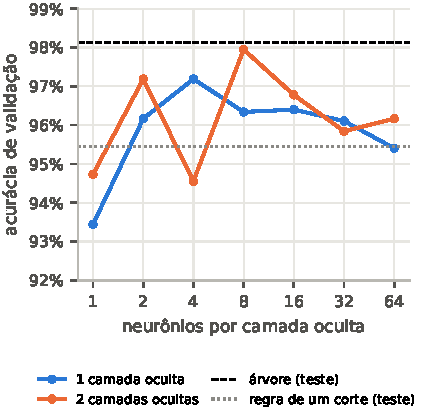
\includegraphics[width=.5\textwidth]{figures/rn_neuronios.pdf}
\caption{Acurácia de validação cruzada (5 partes, seed 42) por número de neurônios em cada camada oculta, com taxa de aprendizado de $10^{-2}$ e sem parada antecipada. As linhas horizontais são a acurácia de teste da árvore e da regra de um corte (média de 10 seeds).}
\label{fig:rn_neuronios}
\end{figure}

\textbf{Épocas e paciência.} Cada época é uma passada completa pelo treino. A Figura~\ref{fig:rn_epocas} acompanha uma rede de 32 neurônios por 400 épocas, sem parada antecipada. A perda de treino continua caindo, enquanto a de validação se estabiliza: a partir daí, a rede passa a ajustar detalhes do treino que não se repetem na validação (Figura~\ref{fig:rn_epocas}a). Com taxa de aprendizado de $10^{-3}$, a rede aprende devagar, e a acurácia de validação passa longos trechos sem melhorar. Com paciência 10, o treino pararia na época \rnParadaLentaDez{}, com \rnParadaAccLentaDez\% de validação, quando a mesma rede chegaria a \rnMelhorLenta\%; com paciência 30, para na época \rnParadaLentaTrinta{}, com \rnParadaAccLentaTrinta\% (Figura~\ref{fig:rn_epocas}b). Com taxa de $10^{-2}$, chega a 97\% em menos de 100 épocas. A busca em grade confirmou o quadro: escolheu a taxa de $10^{-2}$ em \rnSeedsTaxa{} das 10 seeds e duas camadas ocultas em \rnSeedsDuas{} (32 e 16 neurônios em \rnSeedsTrintaDezesseis), e a rede final treinou de \rnEpocasMin{} a \rnEpocasMax{} épocas.

\begin{figure}[ht]
\centering
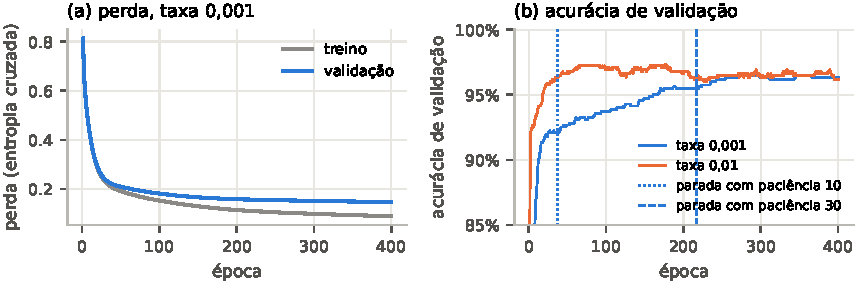
\includegraphics[width=\textwidth]{figures/rn_epocas.pdf}
\caption{Uma rede de 32 neurônios treinada por 400 épocas (seed 42; 80\% do treino para ajustar e 20\% para validar). (a) Perda no treino e na validação, com taxa de aprendizado de $10^{-3}$. (b) Acurácia de validação com as duas taxas; as linhas verticais marcam onde a parada antecipada interromperia a rede de taxa $10^{-3}$ com paciência de 10 e de 30 épocas.}
\label{fig:rn_epocas}
\end{figure}

\textbf{Comparação com os modelos de referência.} A Tabela~\ref{tab:rn_modelos} reúne os seis modelos. A rede acerta \rnAccRede~$\pm$~\rnSdRede\%. Comparando seed a seed, ela supera a regressão logística em todas as 10 seeds (\rnDifRedeLog{} pontos), o que mostra o ganho das camadas ocultas sobre um neurônio só, e supera a regra de um corte em \rnSeedsRedeRegra{} das 10 (\rnDifRedeRegra{} ponto, menos que o desvio entre seeds). Perde para a árvore de decisão em todas as seeds (\rnDifRedeArv{} ponto) e para a Random Forest em 9 (\rnDifRedeRF{} ponto). Também é o modelo menos estável: o desvio de \rnSdRede{} ponto é quase três vezes o da árvore. A AUC conta outra parte da história. A da rede (\rnAucRede\%) é maior que a da árvore (\rnAucArv\%), assim como a da regressão logística (\rnAucLog\%) é maior que a da regra de um corte (\rnAucRegra\%), que acerta mais: os modelos de saída suave ordenam bem os pedidos, e o que erram é o corte em 50\%. Árvore e Random Forest empatam (\rnDifRFArv{} ponto, a floresta melhor em \rnSeedsRFArv{} das 10 seeds).

\begin{table}[ht]
\centering
\caption{Os seis modelos na base de empréstimos (média $\pm$ desvio em 10 seeds; erros em \rnTeste{} pedidos de teste). Tempos: mediana das 10 seeds, num único núcleo. Treino: o do modelo final; busca: a busca em grade com validação cruzada de 5 partes; previsão: os \rnTeste{} pedidos de teste.}
\label{tab:rn_modelos}
\footnotesize
\setlength{\tabcolsep}{4pt}
\begin{tabular}{lccccccc}
\toprule
Modelo & Acurácia (\%) & \shortstack{F1 macro\\(\%)} & AUC (\%) & Erros &\shortstack{Treino\\(ms)} & \shortstack{Busca\\(s)} & \shortstack{Previsão\\(ms)} \\
\midrule
Classe majoritária & 62,2 $\pm$ 0,0 & 38,3 & 50,0 & 323,0 & 0,2 & -- & 0,03 \\
Regra de um corte & 95,5 $\pm$ 0,6 & 95,3 & 96,2 & 38,8 & 1,9 & -- & 0,3 \\
Regressão logística & 91,9 $\pm$ 1,1 & 91,3 & 97,0 & 69,5 & 3,5 & -- & 0,5 \\
Árvore de decisão & 98,1 $\pm$ 0,4 & 98,0 & 98,7 & 16,0 & 3,7 & 0,65 & 0,3 \\
Random Forest & 98,3 $\pm$ 0,4 & 98,2 & 99,8 & 14,5 & 490 & -- & 15,3 \\
Rede neural (MLP) & 96,4 $\pm$ 1,1 & 96,1 & 99,3 & 30,9 & 183 & 23,5 & 0,6 \\
\bottomrule
\end{tabular}

\end{table}

\textbf{Tempo.} Treinar a rede final leva \rnTreinoRedeMs{} ms, cerca de \rnRazaoTreino{} vezes os \rnTreinoArvMs{} ms da árvore, e menos da metade dos \rnTreinoRFMs{} ms da Random Forest. O maior custo da rede está na escolha dos hiperparâmetros: a busca leva \rnBuscaRede{} s por seed, contra \rnBuscaArv{} s da árvore (\rnRazaoBusca{} vezes mais), porque cada uma das \rnCombinacoes{} combinações treina 5 redes por dezenas de épocas. Prever é rápido para quase todos: \rnPrevRedeMs{} ms para a rede e menos de 1 ms para a árvore, contra \rnPrevRFMs{} ms da Random Forest, que consulta 300 árvores.

\textbf{Onde a rede erra.} Na seed 42, a rede comete \rnErrosRedeSeed{} erros no teste, e a árvore, \rnErrosArvSeed. Os erros da rede se concentram logo acima do degrau: entre 550 e 599 pontos há \rnPedidosFaixa{} pedidos de teste, e a rede erra \rnErrosRedeFaixa{}, contra \rnErrosArvFaixa{} da árvore. A árvore, por sua vez, erra sobretudo na exceção dos prazos curtos (score abaixo de 550 e prazo de até 4 anos, \rnExcecao{} pedidos): \rnErrosArvExc{} dos seus \rnErrosArvSeed{} erros, contra \rnErrosRedeExc{} da rede. A Figura~\ref{fig:rn_rampa} mostra a causa. A árvore representa o degrau com uma pergunta e dá probabilidades de 0 ou 100\% em quase todos os pedidos. A rede desenha uma rampa: entre 500 e 599 pontos, \rnInterRede\% das suas probabilidades ficam entre 10\% e 90\%, contra \rnInterArv\% na árvore, e é nessa rampa que estão os seus erros. Redes neurais tendem a aprender funções suaves, e uma relação em degrau é justamente o caso em que modelos de árvore costumam levar vantagem em dados tabulares~\cite{grinsztajn:22}.

\begin{figure}[ht]
\centering
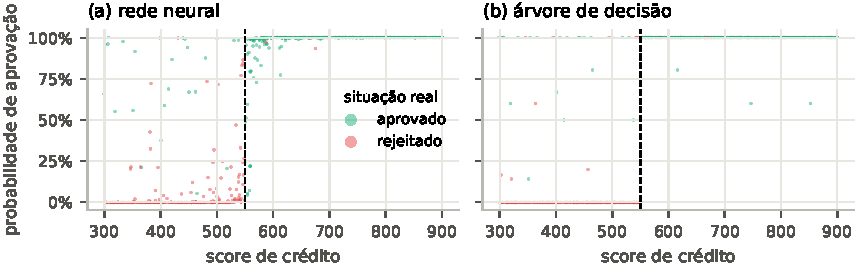
\includegraphics[width=\textwidth]{figures/rn_rampa_degrau.pdf}
\caption{Probabilidade de aprovação prevista para cada pedido de teste, por score de crédito (seed 42), colorida pela situação real. (a) Rede neural. (b) Árvore de decisão. A linha tracejada marca 550.}
\label{fig:rn_rampa}
\end{figure}

\textbf{Tipos de erro.} Com a aprovação como classe positiva, um falso positivo é aprovar um pedido que foi rejeitado, o erro que expõe o banco a calote, e um falso negativo é recusar um pedido que foi aprovado, o que custa um bom cliente. Na seed 42 (Figura~\ref{fig:rn_confusao}), a rede tem \rnFPRedeSeed{} falsos positivos e \rnFNRedeSeed{} falsos negativos; a árvore, \rnFPArvSeed{} e \rnFNArvSeed. Quase toda a diferença está nos falsos negativos, a maioria deles entre 550 e 599 pontos, na rampa da rede. Na média das 10 seeds, porém, a rede erra mais dos dois lados: \rnFPRedeMed{} falsos positivos e \rnFNRedeMed{} falsos negativos por seed, contra \rnFPArvMed{} e \rnFNArvMed{} da árvore. Em proporção, a rede aprova \rnTaxaFPRede\% dos \rnTesteRej{} pedidos rejeitados do teste e recusa \rnTaxaFNRede\% dos \rnTesteAprov{} aprovados (árvore: \rnTaxaFPArv\% e \rnTaxaFNArv\%). Os dois modelos erram mais aprovando do que recusando: só em \rnSeedsFNRede{} das 10 seeds a rede tem mais falsos negativos que falsos positivos, e a árvore também em \rnSeedsFNArv. Se um calote custar mais que um cliente perdido, o corte de 50\% poderia ser elevado, escolhido na validação; não o fizemos, para manter o mesmo critério em todos os modelos.

\begin{figure}[ht]
\centering
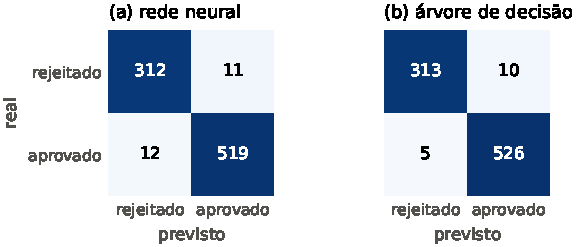
\includegraphics[width=.62\textwidth]{figures/rn_confusao.pdf}
\caption{Matriz de confusão no teste (seed 42, \rnTeste{} pedidos). (a) Rede neural. (b) Árvore de decisão. Cor pela proporção da classe real; número em contagem.}
\label{fig:rn_confusao}
\end{figure}

\section{Limitações}\label{sec:limitacoes}

A principal limitação é a própria base. Distribuições quase uniformes e um rótulo que segue um degrau no score indicam dados sintéticos, gerados por uma regra; em dados de crédito reais, a relação entre os atributos e a aprovação tende a ser mais gradual, o que poderia favorecer a rede. A conclusão de que a árvore vence a rede vale, portanto, para esta base, e não para crédito em geral. A busca da rede cobriu 24 combinações e só o otimizador Adam, e a semente dos pesos iniciais mudou junto com a divisão dos dados, de modo que o desvio entre seeds mistura as duas fontes de variação. Os tempos foram medidos numa única máquina, num núcleo só; os valores absolutos mudam com o computador, e as razões entre modelos são mais estáveis que os tempos em si.

\section{Conclusão e trabalhos futuros}

Na base de \rnLinhas{} pedidos de empréstimo, uma rede neural com padronização e parada antecipada acerta \rnAccRede~$\pm$~\rnSdRede\%: supera a regressão logística, um neurônio só, nas 10 seeds, e a regra de um corte em \rnSeedsRedeRegra{} delas. Sem padronização, ela não aprende (\rnSemPadAcc\%). Com a paciência padrão de 10 épocas e taxa de aprendizado de $10^{-3}$, pararia cedo demais (\rnParadaAccLentaDez\% de validação). Mesmo bem ajustada, a rede perde para a árvore de decisão (\rnAccArv\%) em todas as seeds, treina cerca de \rnRazaoTreino{} vezes mais devagar e exige uma busca de hiperparâmetros \rnRazaoBusca{} vezes mais longa. O motivo é a forma da regra que gerou os rótulos, um degrau no score de crédito: a árvore o representa com uma pergunta, e a rede só o aproxima com uma rampa, onde ficam seus erros. Nesta base, a rede funciona, mas não compensa.

Dois caminhos seguem do que foi visto: repetir a comparação em dados de crédito reais, onde a relação com o score é gradual, e separar a variação causada pelos pesos iniciais da rede da variação causada pela divisão dos dados.


\bibliographystyle{sbc}
\bibliography{refs}

\end{document}
